\newcommand{difficulty}[4] {
    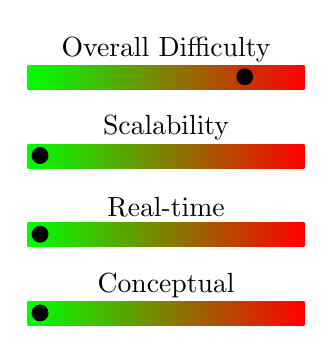
\begin{tikzpicture}%
    \node at (0,3) {Overall Difficulty};%
    \node at (0,2) {Scalability};%
    \node at (0,1) {Real-time};%
    \node at (0,0) {Conceptual};%
    \node [shading = axis,rectangle, left color=green, right color=red,shading angle=90, anchor=north, minimum width=10em, minimum height=2ex] (box) at (0,2.8){};%
    %+/- 1.6%
    \filldraw (\overall,2.65) circle [radius=.1];%
    \node [shading = axis,rectangle, left color=green, right color=red,shading angle=90, anchor=north, minimum width=10em, minimum height=2ex] (box) at (0,1.8){};%
    \filldraw (-1.6,1.65) circle [radius=.1];%
    \node [shading = axis,rectangle, left color=green, right color=red,shading angle=90, anchor=north, minimum width=10em, minimum height=2ex] (box) at (0,0.8){};%
    \filldraw (-1.6,0.65) circle [radius=.1];%
    \node [shading = axis,rectangle, left color=green, right color=red,shading angle=90, anchor=north, minimum width=10em, minimum height=2ex] (box) at (0,-.2){};%
    \filldraw (-1.6,-0.35) circle [radius=.1];%
    \end{tikzpicture}%
}
